\chapter{Technical architecture}
\label{ch:appendix-technical}

\section{Electronic wiring diagram}
\label{sec:appendix-wiring}

Figure~\ref{fig:wiring-schematic} provides the complete electronic wiring schematic for assembly and troubleshooting reference.

The station is centered around a Raspberry Pi Zero 2~W \parencite{rpi-zero-2w}. Three bus distribution headers consolidate the 3.3\,V, 5\,V, and Ground rails to reduce wire congestion. The environmental (SHT35) and multi-spectral (TCS3448) sensors both share a single I$^2$C bus communicating over General Purpose Input/Output (GPIO) 2 (SDA) and GPIO 3 (SCL). The HX711 24-bit analog-to-digital converter is connected via a digital interface over GPIO 5 (DOUT) and GPIO 6 (SCK). The KY-019 relay module controlling the 5\,V COB LED strip is connected to GPIO 23 (BCM). The camera module is connected via a CSI interface directly to the Raspberry Pi.

\begin{figure}[H]
\centering
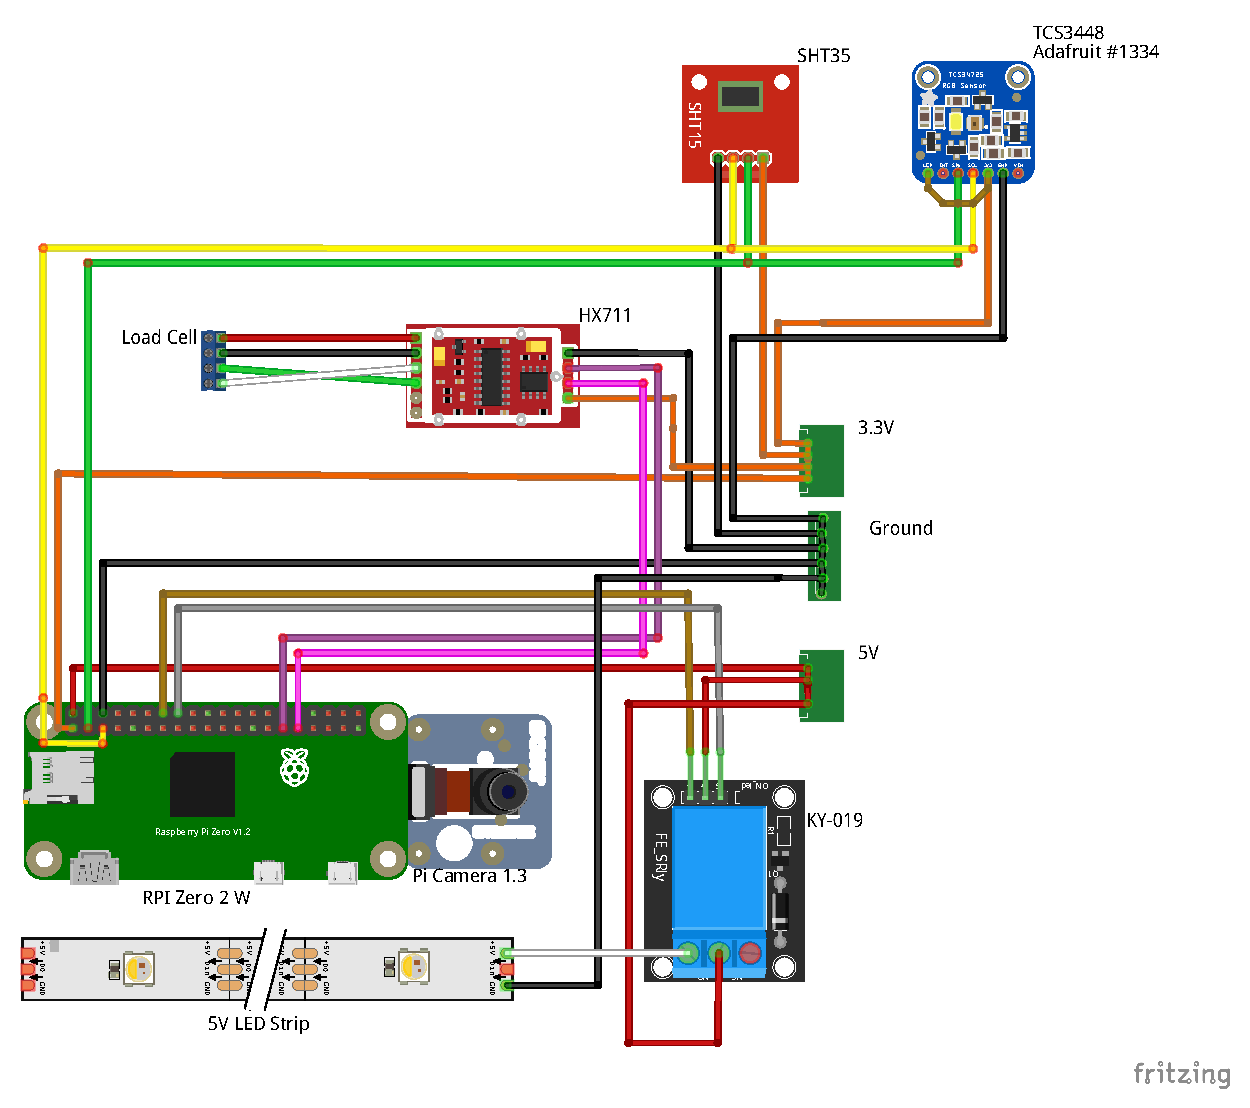
\includegraphics[width=0.95\textwidth]{Images/Wiring_Diagram.pdf}
\caption[PhenoHive Electronic Wiring Schematic]{Complete electronic schematic of the PhenoHive edge sensor station. The Raspberry Pi Zero 2~W is the central compute unit, connected to the SHT35 and TCS3448 over a shared I$^2$C bus, the load cell via an HX711 ADC, the LED relay on GPIO~23 (BCM), and the camera via CSI.}
\label{fig:wiring-schematic}
\end{figure}


\section{3D Printed Casing}
\label{sec:appendix-casing}

The PhenoHive station is housed in a custom designed casing made in CAD and fabricated with a standard 3D printer (Figure~\ref{fig:casing}). The design is available in the project repository under \texttt{casing/}.

The casing is a single continuously printed box with rounded outer corners and four insert holes at the corners for a lid attachment. The interior floor and sides have dedicated mounting pads for each electronic component.


\begin{figure}[H]
    \centering
    \begin{subfigure}[b]{0.52\textwidth}
        \centering
        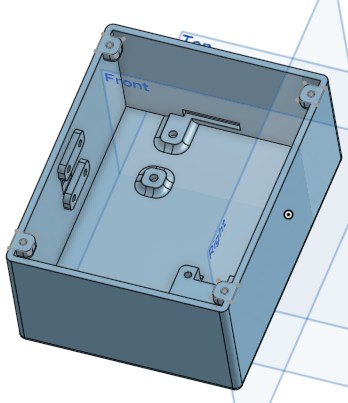
\includegraphics[width=\textwidth]{Images/3d_casing_isometric}
        \caption{Isometric CAD render showing the open-top enclosure, the camera bracket (left wall), and the circular TCS3448 sensor mount on the floor.}
        \label{fig:casing-isometric}
    \end{subfigure}
    \hfill
    \begin{subfigure}[b]{0.44\textwidth}
        \centering
        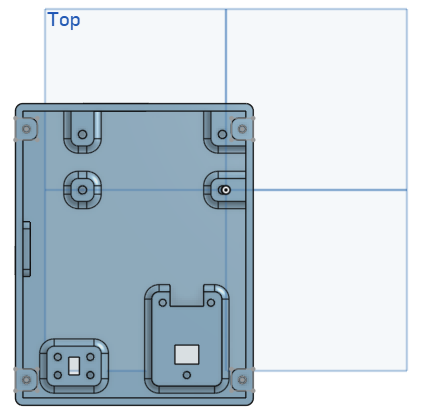
\includegraphics[width=\textwidth]{Images/3d_casing_top}
        \caption{Top-down view that shows the corner screw bosses, the circular sensor seat, the cable routing slot and the breakout board pad.}
        \label{fig:casing-top}
    \end{subfigure}
    \caption[PhenoHive 3D Printed Casing]{CAD renders of the PhenoHive 3D-printed casing. The design enforces a fixed sensor geometry across all stations. All of thefeatures are dimensioned to match the breakout boards listed in the bill of materials (Table~\ref{tab:bom}).}
    \label{fig:casing}
\end{figure}

